\subsection{Examples}



\begin{example2}{Unconditional Branch Flow} The execution starts at line 10.\\
Example of branching sequence and jump table:
\vspace{2mm}\\
1. List the sequence of branch instructions that end in an infinite loop.\\
Do this by stating the branches in tabular form: from - to.\\
E.g. the first branch is $\underline{\mathbf{1 1 - 1 6}}$ (branch unconditionally from line 11 to line 16).
\vspace{2mm}\\
2. At which line does the execution sequence finally loop forever?
\begin{lstlisting}[language=armasm, style=basesmol]
Label1  LDR     R0, =Label5
Label2  BX      R0
Jumptable
        DCD     Case0
        DCD     Case1
        DCD     Case2
        DCD     Case3
Label5  LDR     R0, =Label6
        B       Label2
Label6  LDR     R2, =Jumptable
        ADDS    R2, R2, #4
Label4  LDR     R2, [R2]
        BX      R2
Case0   B       Case0           ; Infinite loop
Case1   LDR     R2, =Jumptable
        MOVS    R1, #3
        LSLS    R1, R1, #2
        ADDS    R2, R2, R1
        B       Label14
Case2   B       Label1
Case3   B       Case0
\end{lstlisting}

\textbf{Solution:}\\
1. Branch sequence:\\ $10-16, 17-11, 11-18, 21-23, 27-20, 21-29, 29-22, 22-22...$\\
2. Loop at line 22
\end{example2}



\begin{example2}{Conditional Branch Flow}
The execution starts at line 10.
\vspace{2mm}\\
1. List which branch instructions jump to the given label.\\
Do this by stating the branches in tabular form: from - to.
\vspace{2mm}\\
2. What is the final value in $R 0$ as hexadecimal value?
\vspace{2mm}\\
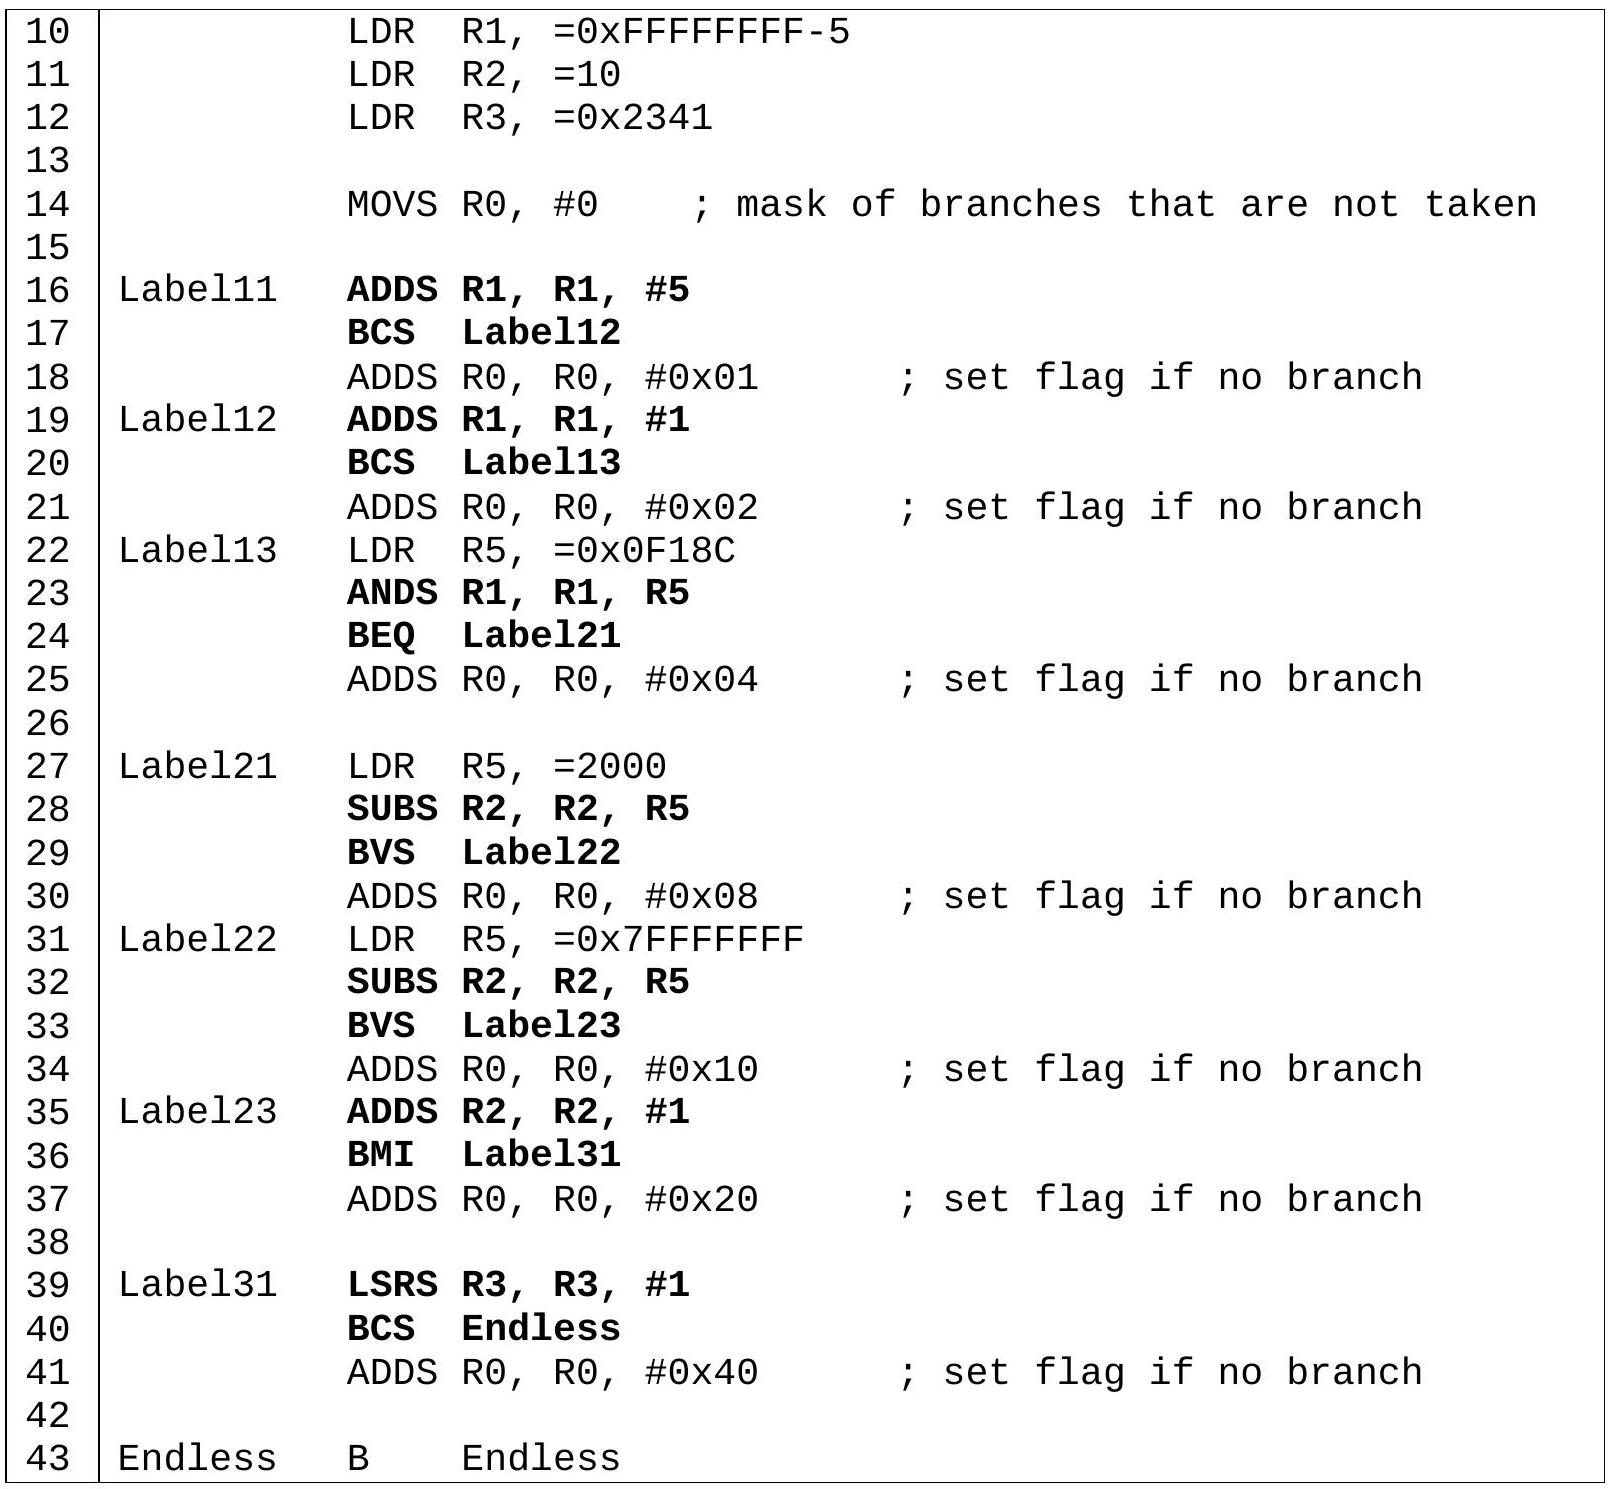
\includegraphics[width=\linewidth]{images/2025_01_02_9902c2d2685de638ef73g-3}


\textbf{Solution:}
\begin{enumerate}
  \item $20-22,24-27,33-35,40-43$
  \item $0 \times 29$ (binary 0010 '1001)
\end{enumerate}
\end{example2}




\begin{example2}{Comparison Instructions}\\
The execution starts at line 10.
\vspace{2mm}\\
1. List which branch instructions jump to the given label.\\

Do this by stating the branches in tabular form: from - to.
\vspace{2mm}\\
2. What is the final value in $R 0$ as hexadecimal value?
\vspace{2mm}\\
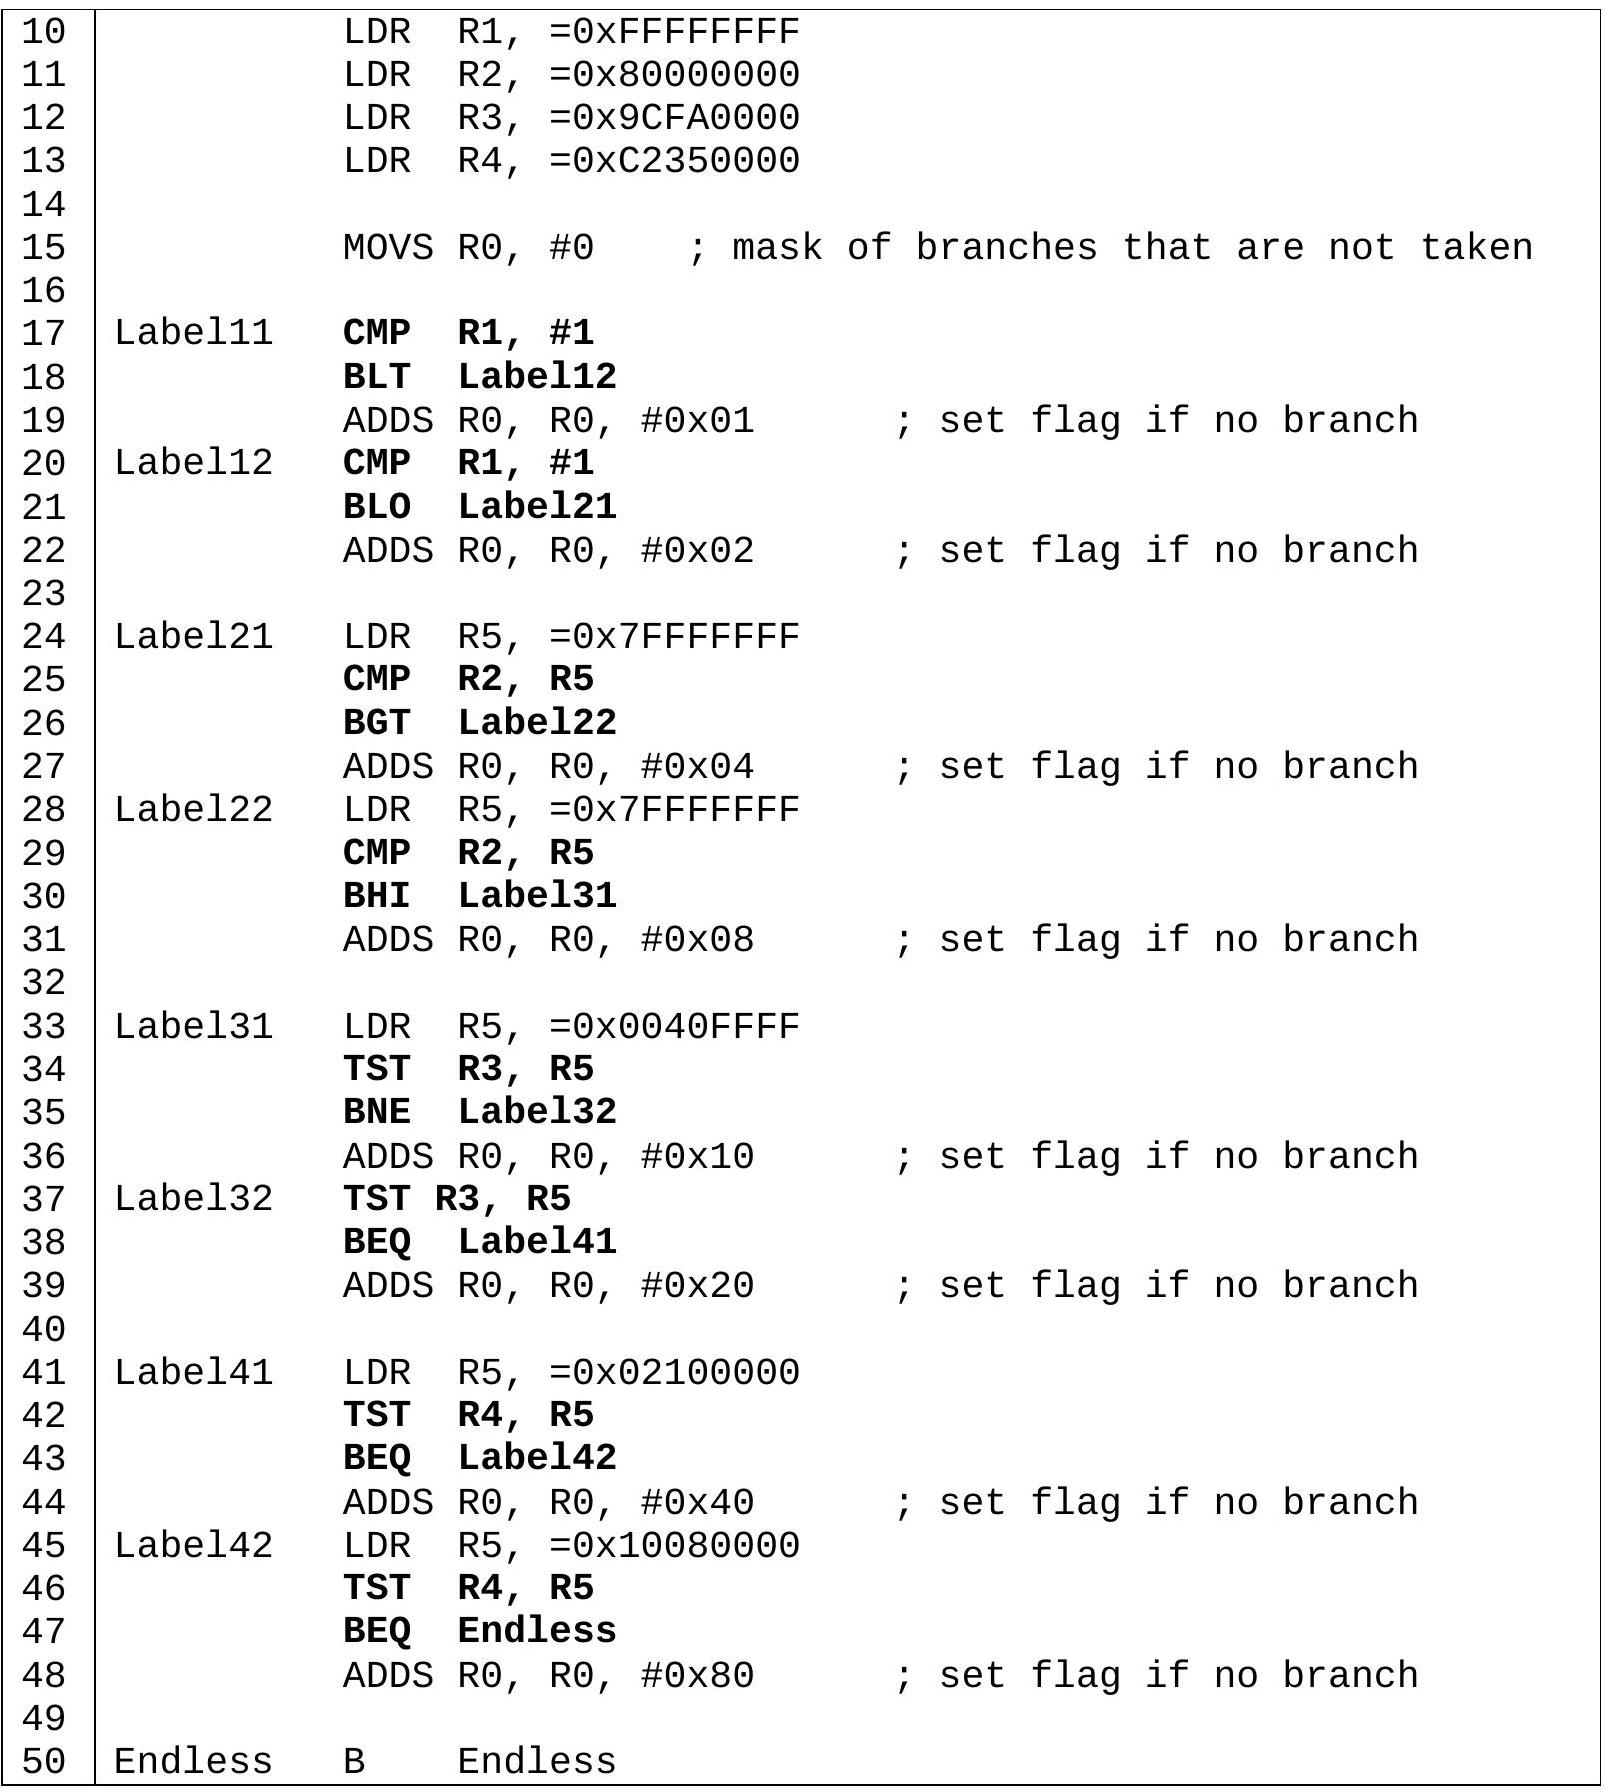
\includegraphics[width=\linewidth]{images/2025_01_02_9902c2d2685de638ef73g-4}

\textbf{Solution:}
\begin{enumerate}
  \item $18-20,30-33,35-37,47-50$
  \item $0 \times 66$ (binary 0110 '0110)
\end{enumerate}
\end{example2}














